% Section content template for individual Educative lessons
% This file contains the actual content for a specific section
% Generated from Educative API section content

% Section: Use Case Diagram for the Movie Ticket Booking System
% Section ID: 5302189004423168
% Section Slug: use-case-diagram-for-the-movie-ticket-booking-system
% Generated: 2025-12-12T14:17:48.524639

Let's build the use case diagram for the movie ticket booking system and understand the relationship between its main actors and functions. First , we'll define the different elements of our system, followed by the complete use case diagram.

\subsection{System}\label{iZoEi88vn7jA-PUgdVkqt}
\\
Our system is the movie ticket booking system. It manages movie and show listings, ticket bookings, seat reservations, and notification delivery.

\subsection{Actors}\label{zRbErjZKFz6Kd1tal5lxu}
\\
Now, we will define the main actors of our movie ticket booking system.

\subsubsection{Primary actors}\label{Ko_2oRm_G-gdHolbZitlm}

\begin{itemize}
\item
\protect\phantomsection\label{8mSrXwj9yCvLyWZTtTvRP}
\textbf{Customer:~} Searches for movies, creates bookings, reserves seats, pays for tickets, views/modifies/cancels bookings.
\item
\protect\phantomsection\label{5FKRfJNiiuwEku6sVCoXC}
\textbf{Ticket agent:}~The ticket agent will assist the customer and perform almost all the tasks a customer can do, such as creating a movie ticket booking on behalf of the customer, searching for movies, and reserving seats at the halls, except for modifying and canceling a booking.
\end{itemize}

\subsubsection{Secondary actors}\label{h0YJQvVfODmpfJo-4IGwx}

\begin{itemize}
\item
\protect\phantomsection\label{Wkaj7wMiOgfgZuMxKMkn_}
\textbf{Admin:}~Manages movies and showtimes by adding, deleting, or updating them.
\end{itemize}

\subsection{Use cases}\label{D9dj_bk8CFBKmWYaCokIb}
\\
This section will define the use cases for movie ticket booking systems. We have listed the use cases according to their interactions with a particular actor.
\begin{quote}
\textbf{Note:} Some use cases will occur multiple times because they are shared among different actors in the system.
\end{quote}
\subsubsection{Admin}\label{pVIi39nDXtJsLCZ1tZClS}

\begin{itemize}
\item
\protect\phantomsection\label{1aUN-I2VbE3U-NdBckerq}
\textbf{Add show:} To add a new show for a particular movie in any cinema hall, specifying the movie, time, hall, and seat layout.
\item
\protect\phantomsection\label{Q6mSSKFqs2MFpgwN26bgp}
\textbf{Modify show:} This function allows you to update the details of an existing show (such as date, time, or hall assignment) for any movie.
\item
\protect\phantomsection\label{Mx-cThz0VKIWCO_zJuolg}
\textbf{Delete (cancel) show:} To remove or cancel a scheduled show for a movie. This may also trigger notifications to affected customers.
\item
\protect\phantomsection\label{ozFfJk1udp2nK50Kmpm7d}
\textbf{Add movie:} To add a new movie to the system's listing, specify the title, language, genre, release date, and description.
\item
\protect\phantomsection\label{GkbBT4qXK_3E6u7_kNj_G}
\textbf{Update movie:} To edit the details of an existing movie, such as title, language, genre, or duration.
\item
\protect\phantomsection\label{qLp5rJUoIT-CuM19K8Zqf}
\textbf{Search movie:} To search for movies in the system using filters like title, language, genre, or release date.
\item
\protect\phantomsection\label{yf5MxcwtkwfgoEQLkqXLr}
\textbf{Delete movie:} To permanently remove a movie from the system, which may also involve canceling all its scheduled shows and notifying customers.
\end{itemize}

\subsubsection{Customer}\label{_Y6YzRRWTz99R6c_8D5mq}

\begin{itemize}
\item
\protect\phantomsection\label{4S8o_hPdPwDqZcm7Atvsj}
\textbf{Search movie:} You can search for movies by title, language, genre, or release date and view available shows across all cinemas.
\item
\protect\phantomsection\label{f3gX5W3xkG7tnT9nM5iDd}
\textbf{Create booking:} To select a show, choose seats from the seating map, provide customer details, and create a booking.
\item
\protect\phantomsection\label{tfexOIdPJHugVdQ7tsOH7}
\textbf{View booking:} To view booking details, including movie name, showtime, cinema, hall, seat numbers, and booking status.
\item
\protect\phantomsection\label{lfL7wFkKYIm-e3FQA1b0c}
\textbf{Modify booking:} To change selected seats or update booking details before final confirmation.
\item
\protect\phantomsection\label{EFwoTpjSHk3UoSD8mWdOf}
\textbf{Cancel booking:} To cancel an existing booking, release reserved seats and, if applicable, request a refund.
\item
\protect\phantomsection\label{y9473rcLTUcVSy34FN-s7}
\textbf{Reserve seat:} To select one or more available seats from the real-time seating map during booking.
\item
\protect\phantomsection\label{Vfi7-eceneZkBbyKqzNhk}
\textbf{Pay for booking:} To complete payment for booked tickets using cash or a credit card (for online bookings).
\end{itemize}

\subsubsection{Ticket agent}\label{Gz1uJtlzFRiNA5tj9jdiG}

\begin{itemize}
\item
\protect\phantomsection\label{FNpsmsfpSSi1V3Gi_O8wk}
\textbf{Search movie:} To search for movies by title, language, genre, or release date, on behalf of a customer at the cinema.
\item
\protect\phantomsection\label{ZIJIL6VOLkiCp_Bnygo-l}
\textbf{Create booking:} To select a show, choose seats, and create a booking for the customer in person.
\item
\protect\phantomsection\label{LqgRAobSnUZEU7oFYYdce}
\textbf{View booking:} To retrieve and display the booking details for a customer at the cinema.
\item
\protect\phantomsection\label{A8GjUOJTJwgFThNLjrzKG}
\textbf{Reserve seat:} To select and reserve available seats for a show during in-person booking.
\item
\protect\phantomsection\label{oyY4f0Z_ggh6FnFw6x8pb}
\textbf{Accept payment:} To collect payment for bookings via cash or credit card on behalf of the customer.
\end{itemize}

\subsubsection{Movie ticket booking system}\label{WIeipQk8lVejblzIqnRBM}

\begin{itemize}
\item
\protect\phantomsection\label{FYNcH2oWBGNspynUdvR-n}
\textbf{Send new movie notification:} To automatically notify users (who have opted in) when a new movie is added to the system.
\item
\protect\phantomsection\label{vY8IvPlGjOAIB8VRNxYjk}
\textbf{Send booking notification:} To send confirmation notifications to customers upon successful booking and payment.
\item
\protect\phantomsection\label{Nn3g1f0wNlYy7urO4zHPu}
\textbf{Send cancellation notification:} Customers should receive notifications if their booking, movie, or show is canceled.
\item
\protect\phantomsection\label{9rxgtCbVp5zx5bqrF1zuF}
\textbf{Send booking modification notification:} To automatically notify customers when their booking details (such as seat selection, showtime, or cinema hall) are changed.
\end{itemize}

\subsection{Relationships}\label{8XbeVkDuJQci_Cl5ti0sA}
\\
This section describes the relationships between actors and use cases in the movie ticket booking system. Understanding these relationships clarifies how different system components interact and helps ensure a robust, consistent design.

\subsubsection{Generalization}\label{vE54YpX_KA9gDKAJUOVIt}
\\
Generalization shows inheritance or specialization between actors or use cases. The Search movie use case generalizes more specific search types:

\begin{itemize}
\item
\protect\phantomsection\label{jJ0v6DNXvJgRwEtvgprVv}
``Search movie by title''
\item
\protect\phantomsection\label{m0JRD8vLOTXvr97ikGn9B}
``Search movie by language''
\item
\protect\phantomsection\label{rFX3V7YTLrM4DBHn3WgbD}
``Search movie by genre''
\item
\protect\phantomsection\label{LdMATf4mHE2DlBKm79UMl}
``Search movie by release date''
\end{itemize}
\\
Each specialized search is a specific way to perform the generic Search movie action. By showing generalization, we communicate that users can choose any of these criteria without changing the main workflow, and future new criteria can be added without restructuring the diagram.

\subsubsection{Associations}\label{1mMjTROkmlHgITsgjnqvo}
\\
The table below shows the association relationship between actors and their use cases.

\begin{center}
{\def\LTcaptype{none} % do not increment counter
\begin{longtable}[]{@{}
>{\raggedright\arraybackslash} p{(\linewidth - 6\tabcolsep) * \real{0.2500}}
>{\raggedright\arraybackslash} p{(\linewidth - 6\tabcolsep) * \real{0.2500}}
>{\raggedright\arraybackslash} p{(\linewidth - 6\tabcolsep) * \real{0.2500}}
>{\raggedright\arraybackslash} p{(\linewidth - 6\tabcolsep) * \real{0.2500}}@{}}
\toprule\noalign{}
\endhead
\bottomrule\noalign{}
\endlastfoot
\begin{minipage}[t]{\linewidth}\raggedright
\textbf{Admin}
\end{minipage} & \begin{minipage}[t]{\linewidth}\raggedright
\textbf{Customer}
\end{minipage} & \begin{minipage}[t]{\linewidth}\raggedright
\textbf{Ticket} \textbf{Agent}
\end{minipage} & \begin{minipage}[t]{\linewidth}\raggedright
\textbf{Movie Ticket Booking System}
\end{minipage} \\
\begin{minipage}[t]{\linewidth}\raggedright
Add show
\end{minipage} & \begin{minipage}[t]{\linewidth}\raggedright
Search movie
\end{minipage} & \begin{minipage}[t]{\linewidth}\raggedright
Search movie
\end{minipage} & \begin{minipage}[t]{\linewidth}\raggedright
Send new movie notification
\end{minipage} \\
\begin{minipage}[t]{\linewidth}\raggedright
Modify show
\end{minipage} & \begin{minipage}[t]{\linewidth}\raggedright
Create booking
\end{minipage} & \begin{minipage}[t]{\linewidth}\raggedright
Create booking
\end{minipage} & \begin{minipage}[t]{\linewidth}\raggedright
Send booking notification
\end{minipage} \\
\begin{minipage}[t]{\linewidth}\raggedright
Delete (cancel) show
\end{minipage} & \begin{minipage}[t]{\linewidth}\raggedright
View booking
\end{minipage} & \begin{minipage}[t]{\linewidth}\raggedright
View booking
\end{minipage} & \begin{minipage}[t]{\linewidth}\raggedright
Send cancellation notification
\end{minipage} \\
\begin{minipage}[t]{\linewidth}\raggedright
Add movie
\end{minipage} & \begin{minipage}[t]{\linewidth}\raggedright
Modify booking
\end{minipage} & \begin{minipage}[t]{\linewidth}\raggedright
Reserve seat
\end{minipage} & \begin{minipage}[t]{\linewidth}\raggedright
Send notifications for booking
\end{minipage} \\
\begin{minipage}[t]{\linewidth}\raggedright
Update movie
\end{minipage} & \begin{minipage}[t]{\linewidth}\raggedright
Cancel booking
\end{minipage} & \begin{minipage}[t]{\linewidth}\raggedright
Accept payment
\end{minipage} & \begin{minipage}[t]{\linewidth}\raggedright
\end{minipage} \\
\begin{minipage}[t]{\linewidth}\raggedright
Search movie
\end{minipage} & \begin{minipage}[t]{\linewidth}\raggedright
Reserve seat
\end{minipage} & \begin{minipage}[t]{\linewidth}\raggedright
\end{minipage} & \begin{minipage}[t]{\linewidth}\raggedright
\end{minipage} \\
\begin{minipage}[t]{\linewidth}\raggedright
Delete movie
\end{minipage} & \begin{minipage}[t]{\linewidth}\raggedright
Pay for booking
\end{minipage} & \begin{minipage}[t]{\linewidth}\raggedright
\end{minipage} & \begin{minipage}[t]{\linewidth}\raggedright
\end{minipage} \\
\begin{minipage}[t]{\linewidth}\raggedright
\end{minipage} & \begin{minipage}[t]{\linewidth}\raggedright
Receive notifications for bookings
\end{minipage} & \begin{minipage}[t]{\linewidth}\raggedright
\end{minipage} & \begin{minipage}[t]{\linewidth}\raggedright
\end{minipage} \\
\begin{minipage}[t]{\linewidth}\raggedright
\end{minipage} & \begin{minipage}[t]{\linewidth}\raggedright
Receive notifications for cancellations
\end{minipage} & \begin{minipage}[t]{\linewidth}\raggedright
\end{minipage} & \begin{minipage}[t]{\linewidth}\raggedright
\end{minipage} \\
\end{longtable}
}
\end{center}

\subsubsection{Include}\label{uWfjdhw1UTNxEsMmfoQFy}
\\
The ``include'' relationship indicates that a use case always incorporates the behavior of another use case into its process.

\begin{itemize}
\item
\protect\phantomsection\label{EPVpqZ9cUV39DJBy1NPOB}
\textbf{Create booking} → \textbf{Reserve seat}:

\begin{itemize}
\item
Reserving seats is essential in the booking process, so ``Create booking'' always includes ``Reserve seat.''
\end{itemize}
\item
\protect\phantomsection\label{jS_ZfbY8HXpjbBmM23ILp}
\textbf{Pay for booking} → \textbf{Send booking notification}:

\begin{itemize}
\item
Sending a booking notification is always included after successful payment.
\end{itemize}
\item
\protect\phantomsection\label{-M7-TZy4_Tud3VSsXcQfc}
\textbf{Cancel booking} → \textbf{Refund payment}:

\begin{itemize}
\item
If payment was made, initiating a refund is always included as part of the cancellation process.
\end{itemize}
\item
\protect\phantomsection\label{Mmdrlh4Hi9d3WCol_x5VI}
\textbf{Add movie} → \textbf{Send new movie notification}:

\begin{itemize}
\item
Notification is always sent when a new movie is added.
\end{itemize}
\item
\protect\phantomsection\label{hsqLE56jZCZAIl2jthnU3}
\textbf{Cancel booking}, \textbf{Delete movie}, \textbf{Delete show} → \textbf{Send cancellation notification}:

\begin{itemize}
\item
Canceling a booking, movie, or show always results in a cancellation notification.
\end{itemize}
\item
\protect\phantomsection\label{Mmdrlh4Hi9d3WCol_x5VI}
\textbf{Modify booking} and \textbf{Modify show} → \textbf{Send booking modification notification}:

\begin{itemize}
\item
Notification is always sent to customers when their booking details (such as seat selection, showtime, or cinema hall) are changed or the admin changes anything regarding the show.
\end{itemize}
\end{itemize}

\subsection{Use case diagram}\label{yg2ds3Z6G6w7qnF0GMFT7}
\\
Here is the use case diagram of the movie ticket management system:

\begin{figure}[htbp]
 \centering
 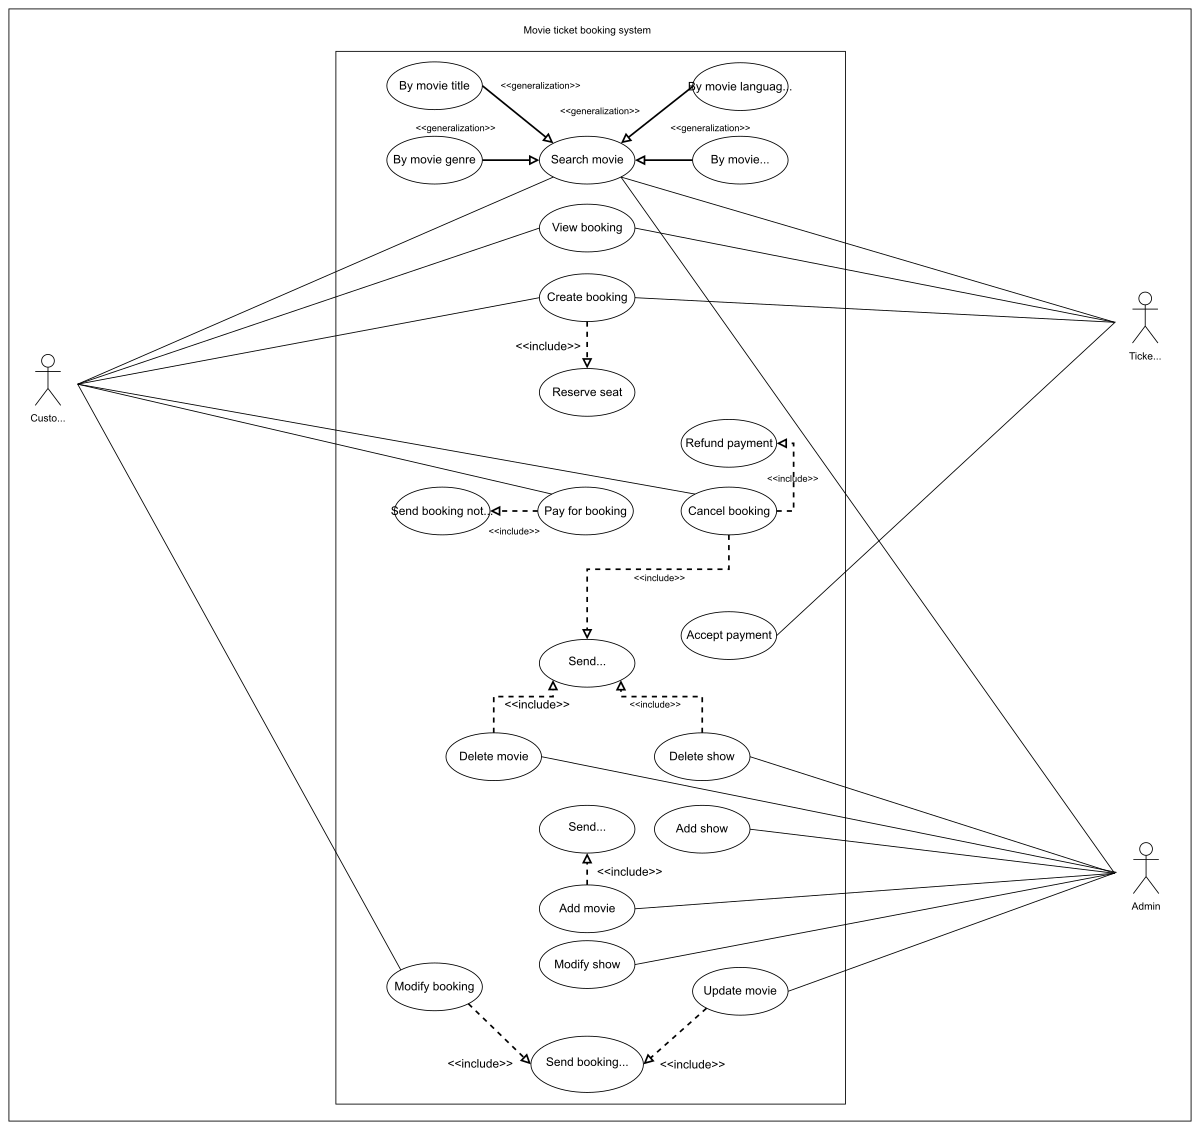
\includegraphics[width=0.5\textwidth]{Images/chapter_14/section_5302189004423168/5080678335905792.png}
 \caption{Use case diagram of a movie ticket booking system}
\end{figure}

In the next lesson, we will discuss the class diagram with a detailed explanation of all classes and their relationship with each other.

% End of section content